\documentclass[11pt]{article}
\usepackage{icmlko}
\begin{document}

\title{계단이지 비탈이 아니다 --- 원핫을 반만 지워도 판은 통째로 지운 만큼 낸다}
\author{월드모델 실험실}
\date{노트 400 · 2026년 8월 1일}
\maketitle

\begin{abstract}
노트 399가 맞바꿈을 값으로 매겼다 --- 도메인 원핫을 빼면 판 $0.0117$ 을
내고 안 본 도메인의 전이를 $+0.2058$ 산다. 이번엔 \textbf{그 값을 치르지
않고 둘 다 갖는} 길을 시험했다. 처방은 드롭아웃이다: 학습 중 행마다 확률
$p$ 로 원핫을 통째로 0 으로 만들면 ``전부 0'' 좌표가 학습 분포 안에 들어와
모형이 거기서 쓸 만한 대비책을 배운다. 사전 등록했다: \emph{$p=0.5$ 면
판은 원핫 있음에 가깝고 전이는 원핫 없음에 가깝다.}

\begin{center}
\begin{tabular}{lrrr}
\hline
드롭아웃 $p$ & KR 만화 & JP 만화 & 판(단일 적합) \\
\hline
$0.00$ (챔피언) & $-0.1261$ & $+0.3196$ & $0.4491$ \\
$0.25$ & $+0.0385$ & $+0.3179$ & $0.4415$ \\
$\mathbf{0.50}$ & $\mathbf{+0.0769}$ & $+0.3173$ & $0.4406$ \\
$0.75$ & $+0.0708$ & $+0.3121$ & $0.4383$ \\
$1.00$ & $+0.0808$ & $+0.3212$ & $0.4387$ \\
\hline
\end{tabular}
\end{center}

\textbf{전이는 맞고 판은 틀렸다.} KR 은 $p{=}0.25$ 에서 벌써 부호를 바꾸고
$p{=}0.5$ 에서 통째 제거($+0.0797$)를 따라잡는다. 그런데 판은
\textbf{$p$ 가 0 을 벗어나는 순간 거의 다 낸다} --- 짝 12뽑기로 $p{=}0.5$
대 챔피언은 $\mathbf{-0.0102 \pm 0.0041}$, \textbf{양수 0/12}. 통째로 뺐을
때가 $-0.0117$ 이었으니 \textbf{반만 지운 값이 아니라 통째로 지운 값}이다.
드롭아웃은 아무것도 사지 못했고, 노트 399의 맞바꿈은 \textbf{전부 0 좌표라는
사고가 아니라 진짜 벽}이다.
\end{abstract}

\section{왜 계단인가}

사전 등록의 셈은 선형이었다 --- 원핫이 절반 살아 있으면 판도 절반만 낸다.
틀렸다. 그림 (나)를 보면 $p{=}0.25$ 에서 이미 $0.4415$ 로 내려앉고 그 뒤로는
$p{=}1.0$ 까지 씨앗 잡음($\pm 0.0033$) 안에서만 움직인다. 원핫이 판에 주는
값은 \textbf{언제나 켜져 있어야} 나오는 종류다. 나무는 갈림에서 그 열을
쓰는데, 그 열이 행마다 무작위로 꺼지면 갈림 자체가 서지 않는다. 4분의 1만
꺼도 그 열은 이미 믿을 수 없는 열이 된다.

이것은 사전 등록의 실패 조건에 그대로 적힌 경우다 --- \emph{판이 원핫 없음
만큼 내려가면 처방이 아무것도 안 산 것이다.}

\section{그런데 값은 어디서 나는가}

판의 $-0.0102$ 가 열한 도메인에 어떻게 흩어지는지 짝지어 갈랐다.

\begin{center}
\begin{tabular}{lrrr}
\hline
도메인 & 유보 행 & 차 & 부호 \\
\hline
아이돌 & $51$ & $-0.1039$ & $0/12$ \\
게임 & $180$ & $-0.0572$ & $0/12$ \\
시장팝업 & $126$ & $-0.0254$ & $3/12$ \\
모바일 & $441$ & $-0.0119$ & $0/12$ \\
펀딩 & $529$ & $-0.0093$ & $1/12$ \\
\hline
세계애니 & $300$ & $+0.0028$ & $10/12$ \\
\textbf{팝업} & $\mathbf{65}$ & $\mathbf{+0.0276}$ & $\mathbf{12/12}$ \\
\hline
\end{tabular}
\end{center}

여기서 만들려던 이야기는 \textbf{``작은 도메인이 원핫으로 절편을 얻는다''}
였다. 아이돌(51행)이 제일 크게 잃고 게임이 그다음이니 그럴듯하다. 그런데
크기와 손해의 순위상관은 $\rho = +0.34$ 밖에 안 되고, \textbf{두 번째로 작은
도메인인 팝업(65행)은 오히려 12/12 로 번다}. 65행이 벌고 51행이 잃는다면
크기가 원인일 수 없다.

\textbf{그래서 값의 출처는 아직 모른다.} 이번 노트가 확정한 것은 값이
\emph{있다}는 것과 그 값이 \emph{쪼개지지 않는다}는 것뿐이다. 원핫은 켜거나
끄거나 둘 중 하나로만 팔린다.

\section{남은 것}

\begin{tabular}{lp{7.6cm}}
\hline
아이돌·게임과 팝업 & 세 도메인이 원핫에서 정반대를 얻는다. 크기가 아니면
무엇인가 --- 축의 결측률? 라벨 퍼짐? 이것이 값의 출처다 \\
도메인 평균만 따로 & 원핫이 나르는 것이 절편뿐이라면 평균을 열 하나로 주고
원핫은 빼 본다. 그 열은 모르는 도메인에서도 정의된다 \\
세 번째 전이 짝 & CN 만화 2025+ 19행 --- 더 모으거나 다른 도메인 \\
\hline
\end{tabular}

\begin{figure}[h]
\centering
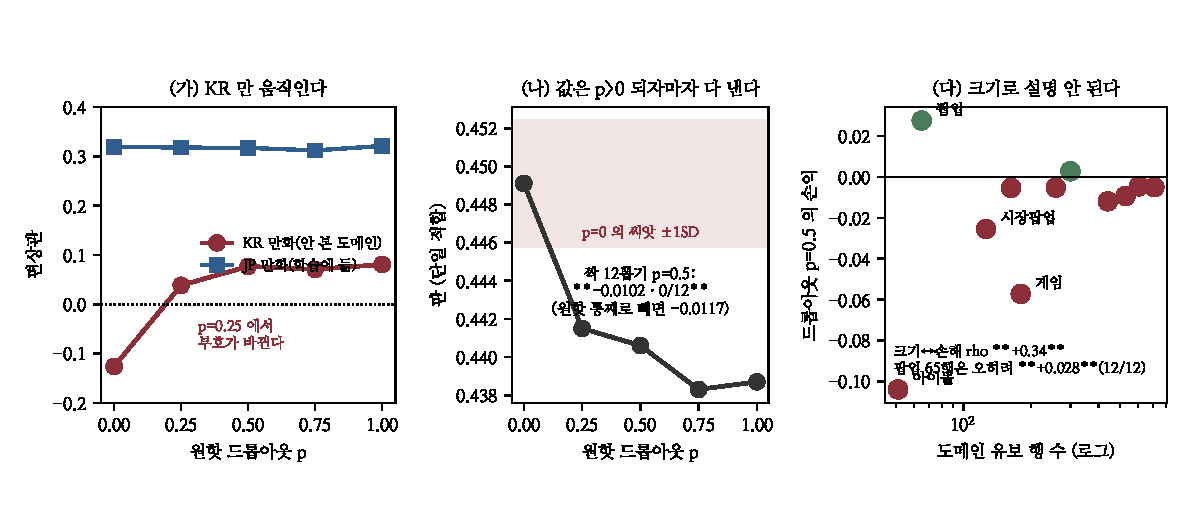
\includegraphics[width=\textwidth]{figs/fig400.pdf}
\caption{(가) 드롭아웃은 안 본 도메인만 움직인다 --- KR 은 $p{=}0.25$ 에서
부호를 바꾸고, 학습에 든 JP 는 $p$ 전 구간에서 평평하다. (나) 판은 $p$ 가
0 을 벗어나는 순간 거의 다 낸다 --- 비탈이 아니라 계단. 띠는 $p{=}0.0$ 의
씨앗 $\pm 1$SD. (다) 손해는 도메인 크기로 설명되지 않는다 --- 팝업 65행이
$+0.028$ 로 12/12 를 번다.}
\end{figure}

\end{document}
